\documentclass[a4paper,12pt]{report}
\usepackage[utf8]{inputenc}
\usepackage{amsmath}
\usepackage{graphicx}
\usepackage{listings}
\usepackage{tikz}
\usepackage[T1]{fontenc}
\usepackage{color}
\usetikzlibrary{arrows,automata}
\definecolor{pythonred}{rgb}{0.6,0,0} % for strings
\definecolor{pythongreen}{rgb}{0.25,0.5,0.35} % comments
\definecolor{pythonpurple}{rgb}{0.5,0,0.35} % keywords
	\definecolor{pythondocblue}{rgb}{0.25,0.35,0.75} % javadoc
	 
	\lstset{language=python,
	basicstyle=\ttfamily,
	keywordstyle=\color{pythonpurple}\bfseries,
	stringstyle=\color{pythonred},
	commentstyle=\color{pythongreen},
	morecomment=[s][\color{pythondocblue}]{/**}{*/},
	numbers=left,
	numberstyle=\tiny\color{black},
        stepnumber=2,
	numbersep=10pt,
	tabsize=4,
	showspaces=false,
	showstringspaces=false}

% Title Page

 \title{\bfseries\huge \textcolor{purple}{\underline {EEP702-Software Lab}} \\{\textcolor{blue}{Assignment7 : Sentiment Analysis in Python}}}
\author{\bfseries\large\textcolor{black}  {Harshit Kumar Gupta}\\ {\textcolor{black} {2013EET2369 }}\\

\includegraphics[width=3cm,height=3.4cm]{./iit.png}\\\noindent Computer Technology\\
\noindent Department Of Electrical Engineering\\IIT DELHI}
% iit.png: 282x282 pixel, 72dpi, 9.95x9.95 cm, bb=0 0 282 282
\begin{document}
\maketitle
\tableofcontents

\begin{center}
 \chapter{\textcolor{blue}{\underline {PROBLEM STATEMENT}}}
\noindent Write a program in Python as per the given statement.

\begin{enumerate}
 \item You are given a text file which contains random facebook status.
 \item You have to do sentiment analysis of those posts on the basis of
       positive,negative and neutral feelings.
 \item To differentiate between feelings, create a dictionary having various positive and
negative words.
\item Match whether a post has any of those words and if it has, it gets counted into the
respective category.Also Include emoticons (for ex. :) for positive and :( for sad).
\item Consider a post having neither positive nor negative feelings as neutral.
\item TASKS
\begin{enumerate}
 \item Count the number of posts with each kind of ‘feeling’ for a given hour (use
a command line tool).
\item Make a table with entries “feeling” and “its count in terms of posts in a
given hour”
\item For each hour,normalize this counted data on the scale of [-1,0,1] i.e.
assign weight of -1 to negative feeling, +1 to positive feeling , 0 to neutral
feeling and adding all, divide result by total number of posts in that
hour.From this calculated data, plot a graph with hour as X-axis and
normalized feeling value as Y-axis.
\end{enumerate}
\item Find the respective hours in which most number of posts arrived for each category of
feeling.
\item Given any two “geographically separate” places, compare the number of posts in those
places containing different category of feelings.
\item Extract the location of the places in the post and give a graphical representation with the
place as X-axis and the normalized mood value for the whole file on Y-axis.


\end{enumerate}

\end{center}

\begin{center}
\chapter{\textcolor{blue}{\underline {ABSTRACT}}}
\end{center}
\noindent The Intention of the Python Code is to practice and get familiar with the python programming. Sentiment analysis or opinion mining is the computational study of people’s opinions,
sentiments, attitudes, and emotions expressed in written language. It is one of the most active research
areas in natural language processing and text mining in recent years. Its popularity is mainly due to two
reasons. First, it has a wide range of applications because opinions are central to almost all human
activities and are key influencers of our behaviors. Whenever we need to make a decision, we want to
hear others’ opinions. Second, it presents many challenging research problems, which had never been
attempted before the year 2000.
\begin{center}
\chapter{\textcolor{blue}{\underline {INTRODUCTION}}}
\end{center}
\noindent Python is a widely used general-purpose, high-level programming language. Its design philosophy 
emphasizes code readability, and its syntax allows programmers to express concepts in fewer lines of code than would 
be possible in languages such as C. The language provides constructs intended to enable clear programs on both
a small and large scale

Python supports multiple programming paradigms, including object-oriented, imperative and functional programming or 
procedural styles. It features a dynamic type system and automatic memory management and has a large and comprehensive
standard library.

Sentiment analysis (also known as opinion mining) refers to the use of natural language processing, text analysis and
computational linguistics to identify and extract subjective information in source materials.

Generally speaking, sentiment analysis aims to determine the attitude of a speaker or a writer with respect to some 
topic or the overall contextual polarity of a document. The attitude may be his or her judgment or evaluation 
(see appraisal theory), affective state (that is to say, the emotional state of the author when writing), or the 
intended emotional communication (that is to say, the emotional effect the author wishes to have on the reader).

\begin{center}
\chapter{\textcolor{blue}{\underline {SPECIFICATIONS AND ASSUMPTIONS}}}
\end{center}
\section*{Specifications}

\begin{enumerate}
\item Different Functions have been used for different objectives.
\item Show function is used to display the answers.


\end{enumerate}

\section*{Assumptions}

\begin{enumerate}
\item There is new line and time stamp between two comments.

\item The time is input as hh:mmam/pm.
\item The file is in utf-8 format.

\end{enumerate}
 
\begin{center}
\chapter{\textcolor{blue}{\underline {LOGIC USED/METHODOLOGY}}}
\end{center}
The methodology that is used for developing the program is defined below:\\

\begin{enumerate}
\item We intiate our code in Python by importing the required libraries.
\item We input the data.txt file and extract the post, time and place and store all the data.
\item Now we create a dictionary with positive and negative words.

\item Next we compare the post with the dictionary and calculate the positive and negative words in every post
\item We normalize the positive and negative words data and plotted graph between hour and normalize value.
\item The values are recorded into a file system.
\item further Searching of the values done from the file named data.txt
\item Records may be deleted added as per specification.

\end{enumerate}


\begin{center}
\chapter{\textcolor{blue}{\underline {EXECUTION INSTRUCTIONS}}}
\end{center}
\begin{enumerate}
 \item For program following instructions are used.
 \begin{enumerate}
  \item python sentiment.py
 \end{enumerate}

\end{enumerate}

\begin{center}
\chapter{\textcolor{blue}{\underline {RESULTS AND CONCLUSIONS}}}
\end{center}
\noindent For the given set of inputs the program exactly displays the Library management Database.\\
\begin{center}
 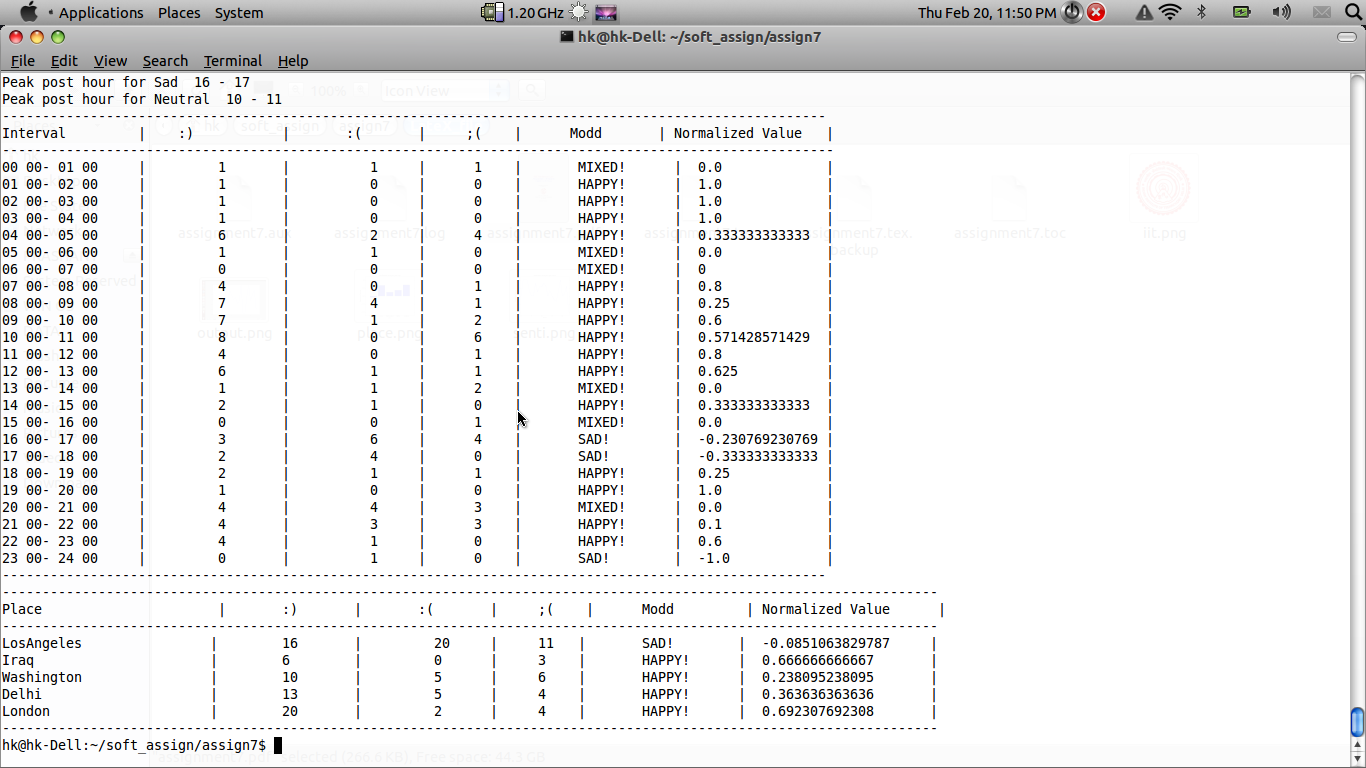
\includegraphics[width=13 cm,height=12 cm]{./Screenshot.png}
 % output.png: 1280x800 pixel, 72dpi, 45.16x28.22 cm, bb=0 0 1280 800
\end{center}
\begin{center}
 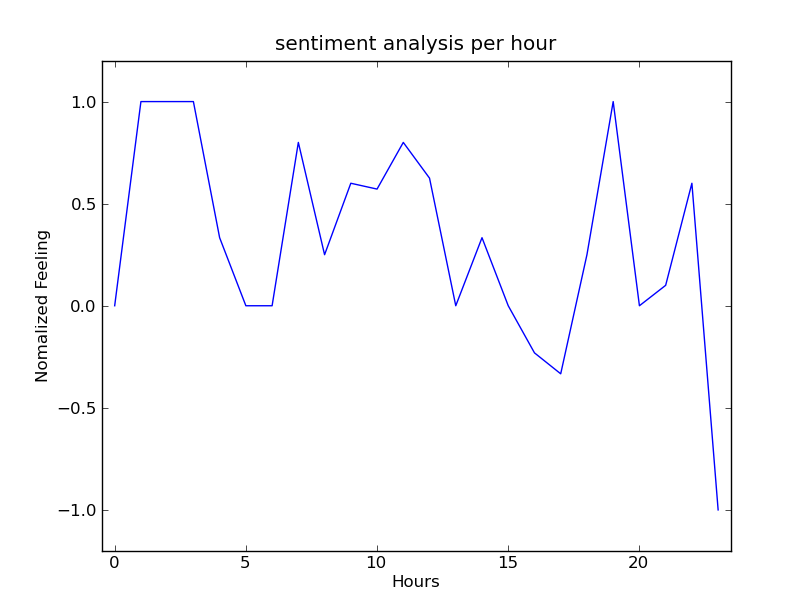
\includegraphics[width=13 cm,height=12 cm]{./senti.png}
 % output.png: 1280x800 pixel, 72dpi, 45.16x28.22 cm, bb=0 0 1280 800
\end{center}
\begin{center}
 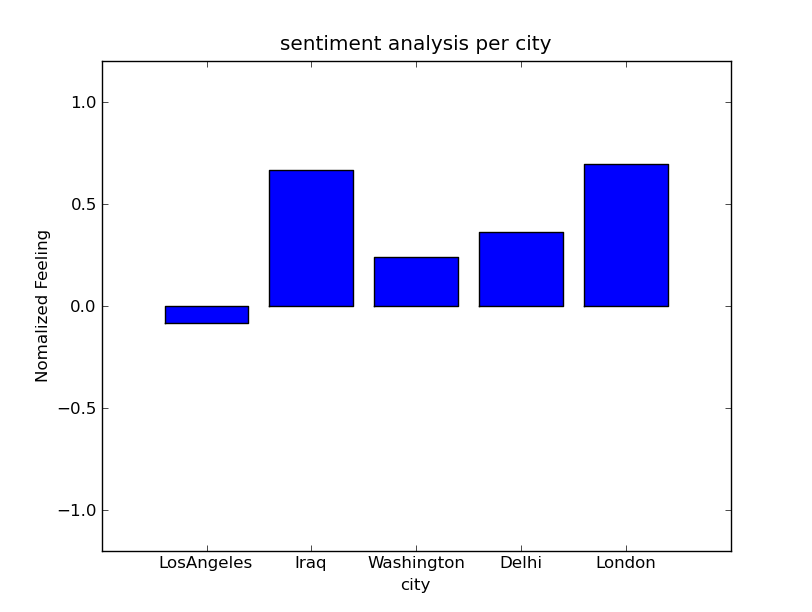
\includegraphics[width=13 cm,height=12 cm]{./place.png}
 % output.png: 1280x800 pixel, 72dpi, 45.16x28.22 cm, bb=0 0 1280 800
\end{center}
\end{document}  
